\section{Example of Applying Framework}
\label{sec:example_applications}

We illustrate the application of Equation (\ref{eq:general_scal}) using an $N$-node TDMA network with three different topologies: clique, line, and grid, also known as a ``Manhattan grid.''  Discussion of other network control protocols and topologies are addressed in Section \ref{sec:discussion}.  We adopt a traffic model that uses Top-K queries as an example application.  We assume that all nodes have a set of collected images that are used to respond to Top-K queries.  Each node produces queries according to a Poisson process with exponential interarrival times with parameter $\lambda$, each with a target image and target QoI, $\mathbf{q} = \{C, T\}$, describing the required completeness (here, we use sum similarity) and timeliness, and sends it to another node chosen at random.  Here, the actual size of the response fulfilling the query can be given by a distribution that incorporates the number of images required, $k_{req}$, and the size of each image.  The details of this distribution can be given from empirical observations of experiments like those in Section \ref{sec:qoi_model}.

\begin{table*}[]
\centering
\begin{tabular}{l|l|l|l|l|l|}
\cline{2-6}
%                            					 & \boldmath{$CF$}  			& \boldmath{$TF_{\mu}$}   			& \boldmath{$TF_{\sigma}$}										& \boldmath{$DF$}			& \boldmath{$PL_{max}$}	\\ \hline
                            					 & \boldmath{$CF$}  			& \boldmath{$\mu_{TF}$}   			& \boldmath{$\sigma_{TF}$}										& \boldmath{$DF$}			& \boldmath{$PL_{max}$}	\\ \hline
\multicolumn{1}{|l|}{\textbf{Clique}} 	& $N-1$ 						& $1$                            				& $0$                            												& $1$  						& $1$ 					\\ \hline
\multicolumn{1}{|l|}{\textbf{Line}}   	& $3$   							& $\frac{N-1}{2}$ 					& $\sqrt{\frac{N-1}{2}}$ 		& $1.5$						& $N-1$				\\ \hline
\multicolumn{1}{|l|}{\textbf{Grid}}   	& $5$   							& $\sqrt{N}$                       			&$N^{\frac{1}{4}}$							&  $2.5$					& $2 \cdot \sqrt{N}$   	\\ \hline
\multicolumn{1}{|l|}{\textbf{NSFNET}}  & $4$  & $2.15$  &$1.47$ &  $2$  & $4$  \\ \hline
\end{tabular}
\vspace{1mm}
\caption{CF, TF, DF, and PL values for example topologies}
\label{table:rf_ff_sf_values}
\end{table*}

\subsection{Scalability Equations}

We outline details on how to derive an expression for the Traffic Factor ($TF$) of a network in Appendix \ref{sec:derivation_TFs}. The result from that process is a mean and standard deviation of a distribution for the traffic factor. In the case of uniform network structures that are scalable, these expressions depend on the network size $N$. For fixed-size networks with a given topology, such as the NSFNET network in Figure \ref{fig:NSF_net} (also in Appendix \ref{sec:derivation_TFs}), the distribution is given with values calculated using the topology and traffic pattern. 

Once an expression for the Traffic Factor ($TF$) is derived, we can use it along with expressions for the Channel Factor ($CF$), Delay Factor ($DF$), and Path Length ($PL$) for the network to create specific instances of Equation (\ref{eq:general_scal}) that estimate the scalability and QoI-satisfiability limits of the particular network of interest.  Since our goal is to determine the point at which the system is unable to support the offered traffic load within the timeliness constraints, we use maximum values for these factors where applicable, specifically $TF_{max}$ and $PL_{max}$. 

\begin{table*}[]
\centering
\begin{tabular}{l|l|}
\cline{2-2}
                             & \multicolumn{1}{c|}{{\bf Equation}} \\ \hline
\multicolumn{1}{|l|}{\textbf{Clique}} & \multicolumn{1}{c|}{$W \cdot T - I_S \cdot k_{req} \cdot (N-1) \geq 0$}            \\ \hline
\multicolumn{1}{|l|}{\textbf{Line}}   & \multicolumn{1}{c|}{$W \cdot T - 3 \cdot I_S \cdot k_{req} \cdot (\frac{N-1}{2} + (\frac{-\ln(\epsilon)}{N-1} \pm \sqrt{\frac{\ln(\epsilon)^2}{(N-1)^2} - 4\frac{\ln(\epsilon)}{N-1}} ) \cdot \frac{N-1}{2}) - 1.5 \cdot P_S \cdot (N-1) \geq 0$}       \\ \hline
\multicolumn{1}{|l|}{\textbf{Grid}}   & \multicolumn{1}{c|}{$W \cdot T - 5 \cdot I_S \cdot k_{req} \cdot ( \sqrt{N} + (\frac{-\ln(\epsilon)}{2\sqrt{N}} \pm \sqrt{\frac{\ln(\epsilon)^2}{4 \cdot N} - 2\frac{\ln(\epsilon)}{\sqrt{N}}} ) \cdot N^{\frac{1}{4}}) - 2.5 \cdot P_S \cdot (2 \cdot \sqrt{N} - 1) \geq 0$}      \\ \hline
\multicolumn{1}{|l|}{\textbf{NSFNET}}   & \multicolumn{1}{c|}{$W \cdot T - 4 \cdot I_S \cdot k_{req} \cdot ( 2.15 + (\frac{-\ln(\epsilon)}{2 \cdot 2.15} \pm \sqrt{\frac{\ln(\epsilon)^2}{4 \cdot 2.15^2} - 2\frac{\ln(\epsilon)}{2.15}} ) \cdot 1.47) - 2 \cdot P_S \cdot 4 \geq 0$}      \\ \hline
\end{tabular}
\vspace{1mm}
\caption{Scalability equations}
\label{table:scal_eqs}
\end{table*}

The $PL_{max}$ is usually quickly determined by an examination of the topology, such as $PL_{max} = N-1$ for a line network and $PL_{max} = 2 \cdot \sqrt{N}$ for a grid network.  In some cases, such as the example in Section \ref{sec:scal_feasible_qoi}, a direct value of $TF_{max}$ may be clear from the topology and application.  When traffic is stochastic, though, as it is in this case, we can utilize the distribution of $TF_b$ to capture the expected maximum value of $TF$ with a probability of $(1-\epsilon)$.  If we use a normal distribution for $TF$, then $TF_{max} = \mu_{TF} + \eta \cdot \sigma_{TF}$ where $\eta$ is chosen to satisfy the desired value of $\epsilon$.  This notion is analogous to the z-score of a standard normal distribution.  As an example, using $\eta = 3.5$ captures approximately $99.7\%$ of the maximum of the $TF$ distribution, providing an estimate within $\epsilon = 0.03$ of the maximum probability.  When the Poisson distribution is used to approximate $TF$, we can use a Chernoff bound to provide the $TF_{max}$ expression.  
%Here, we use the multiplicative Chernoff bound\renewcommand{\thefootnote}{\arabic{footnote}}\footnote[1]{This bound can be easily proved using the same outline of the proof used to bound cases for $0 < \eta \leq 1$ in \cite{mitzenmacher2005probability}.}, assuming $\eta > 1$:
Here, we use the following multiplicative Chernoff bound (proof of this bound is in Appendix \ref{sec:chernoff_bound_proof}): 
Assuming $\eta > 1$,
\begin{equation}
\label{eq:chernoff_bound}
  P( TF \geq (1 + \eta)\mu_{TF} ) \leq e^{\frac{-\eta^2}{2+\eta}\mu_{TF}}
\end{equation}
Setting the RHS side of (\ref{eq:chernoff_bound}) equal to $\epsilon$ and solving for $\eta$, we get the following expression, which should have real, non-negative roots for small $\epsilon$ values:
\begin{equation}
  \eta = \frac{-\ln(\epsilon)}{2\mu_{TF}} \pm \sqrt{\frac{\ln(\epsilon)^2}{4\mu_{TF}^2} - \frac{2\ln(\epsilon)}{\mu_{TF}}}
\end{equation}

% simply utilize the mean and standard deviation of the distribution derived above to create the following: $TF_{max} = \mu_{TF} + \eta \cdot \sigma_{TF}$ where $\eta$ is a factor that can adjust how conservative the estimates should be.  This notion of $\eta$ is analogous to the z-score of a standard normal distribution, and is applicable here since $TF_x$ approaches a Normal distribution as the network size, $N$, grows.  As an example, we use $\eta = 3.5$ in the validation results below, which captures approximately $99.7\%$ of the maximum of the $TF$ distribution.  

Table \ref{table:rf_ff_sf_values} shows expressions for factors representing general clique, line, and grid networks as well as the NSFNET network as derived in Appendix \ref{sec:derivation_TFs} and in \cite{symptotics_journal}. Then, substituting the factors into equation \ref{eq:general_scal}, we achieve the scalability equations for each topology in Table \ref{table:scal_eqs}.  


To find the limitation of a particular parameter or QoI component, the scalability equation can be solved for the variable of interest.  Then all known values can be substituted to get the limit of the variable of interest.  For example, given a network size and completeness requirement, we can determine a clique network's minimum sustainable timeliness with the equation $T  \geq \frac{I_S \cdot k_{req} \cdot (N-1)}{W}$, where $k_{req}$ is given by the completeness function $Q(C)$.  In practice, solutions for these equations will most likely need to be made numerically, but doing so is rather straightforward using any number of commonly available tools and is much faster and simpler than developing and running separate simulations to determine scalability.  Additionally, as we will show in Section \ref{sec:network_design}, these equations can also be easily used to determine the impact of other network parameters on this timeliness limit. 

\subsection{Minimum Timeliness/Maximum Query Rate}

Solving the Scalability equations for $T$ reveals the minimum satisfiable timeliness value for which all queries are expected to complete within the deadline constraint, which we will call $T_{min}$.  Consequently, this minimum satisfiable timeliness value also correlates to the maximum traffic rate that can be served by the network, $\lambda_{max} = \frac{1}{T_{min}}$.  If the average rate of queries, $\lambda$, is greater than $\frac{1}{T_{min}}$, then the traffic will exceed the network capacity and the number of active queries in the system will grow without bound, causing packets to be dropped and/or delays to grow without bound.  Therefore, the maximum query rate per node is $\lambda_{max} = \frac{1}{T_{min}}$, and, consequently, the minimum timeliness for which \emph{all} flows can be expected to complete before the deadline is $T_{min}$.

%To determine maximum expected delay, $d_{max}$, of a flow in the network, which occurs at the delay $d$ at which $F_{D}$ reaches its maximum value of $1$.  If the average rate of queries, $\lambda$, is greater than $\frac{1}{d_{max}}$, then the traffic will exceed the network capacity and the number of active queries in the system will grow without bound, causing packets to be dropped and/or delays to grow without bound.  Therefore, the maximum query rate is $\lambda_{max} = \frac{1}{d_{max}}$, and, consequently, the minimum timeliness for which \emph{all} flows can be expected to complete before the deadline is $d_{max}$.

In some applications, having a certain amount of queries not complete by the timeliness requirement may be acceptable.  As we show in Section \ref{sec:delay_char}, we can develop a more detailed characterization of the delay equation than the Scalability Equations here for these applications. 
%In some applications, having a certain amount of queries not complete by the timeliness requirement may be acceptable.  In these situations, more useful information can be extracted from the delay distribution in Equation (\ref{eq:full_delay_cdf}).  Specifically, this delay distribution can be interpreted as the expected percentage of queries that will finish within the timeliness constraint if the timeliness constraint was $d$.  As we will show in Section \ref{sec:example_applications}, this relationship follows a Normal distribution CDF.

\subsection{Validation of Scalability Equations}
\label{sec:validation}

\begin{figure}[]
\centering
       \subfigure[Line Network, $I_S = 18 KB$]{
        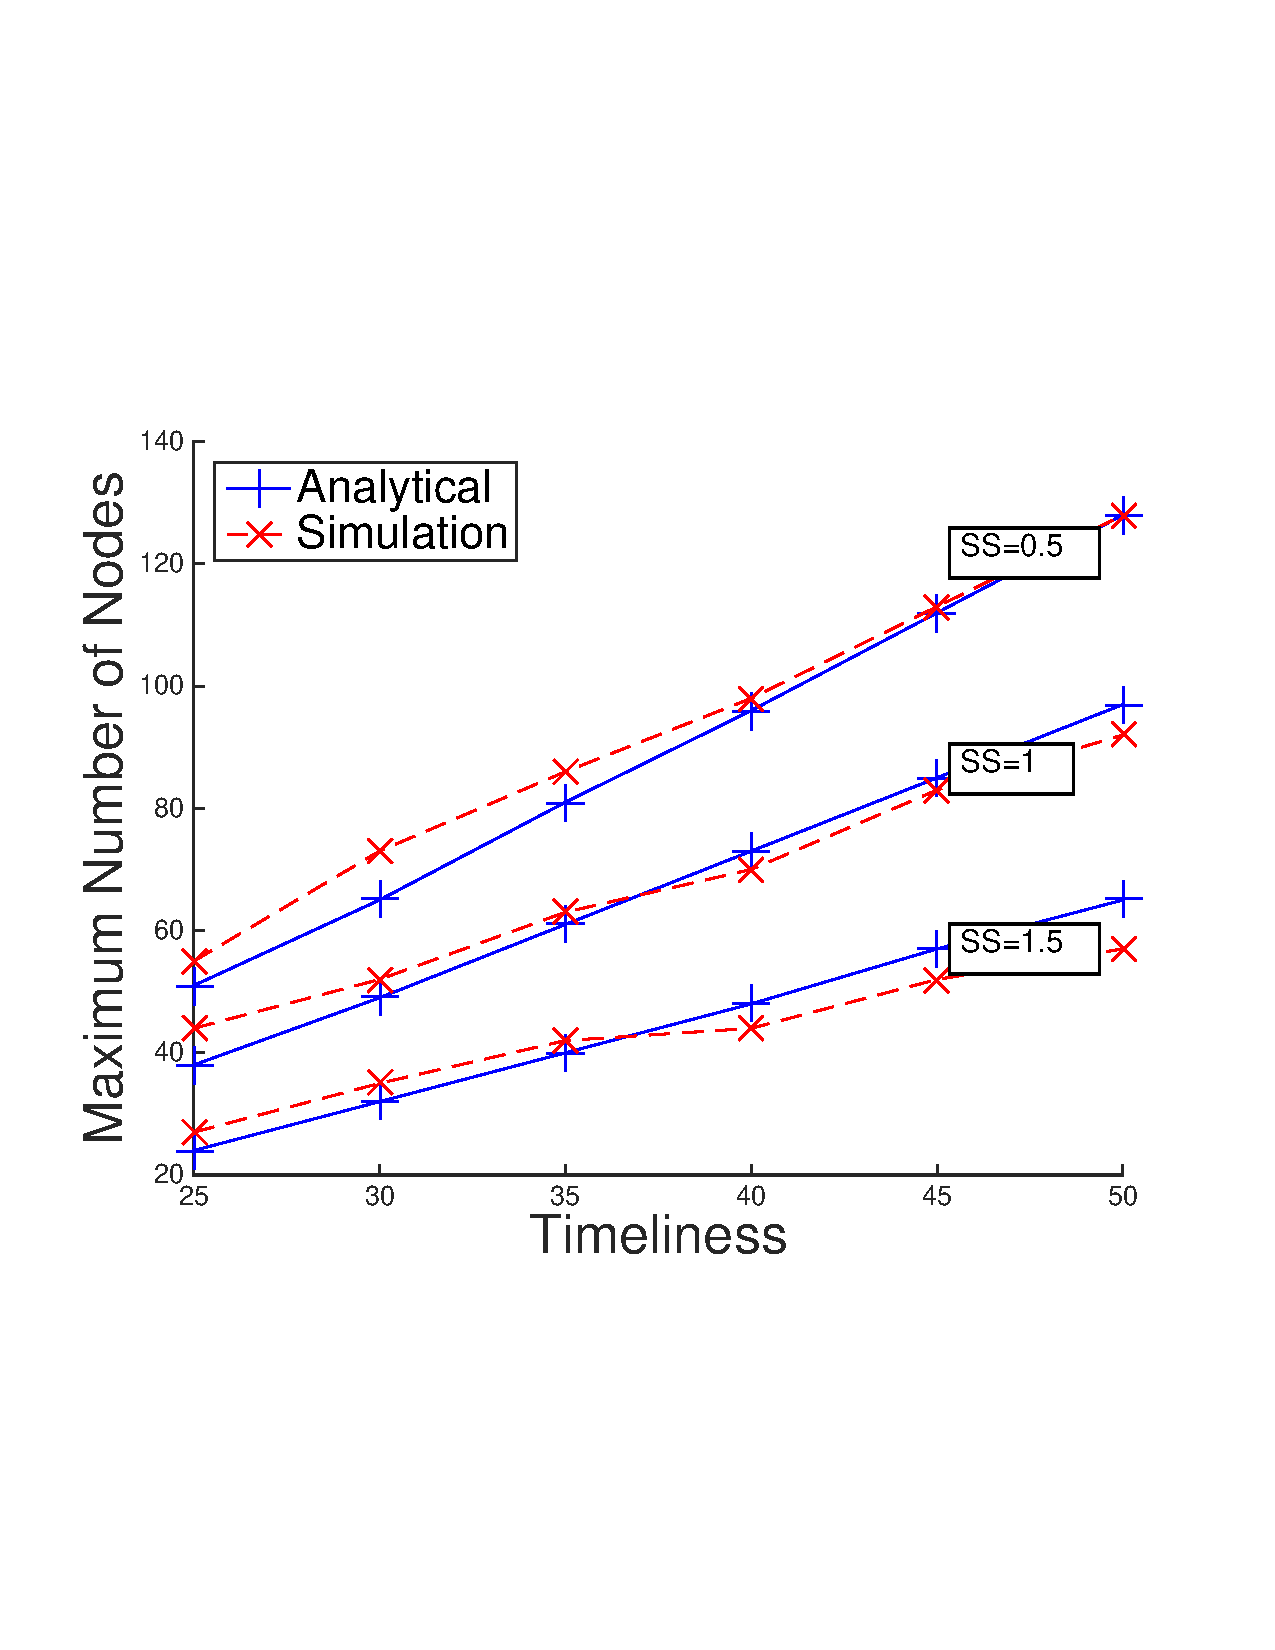
\includegraphics[scale=0.40, clip=true, trim=12mm 65mm 20mm 65mm]{figures/scal_sim_results/color_2d/line_scal_chernoff.pdf}
%        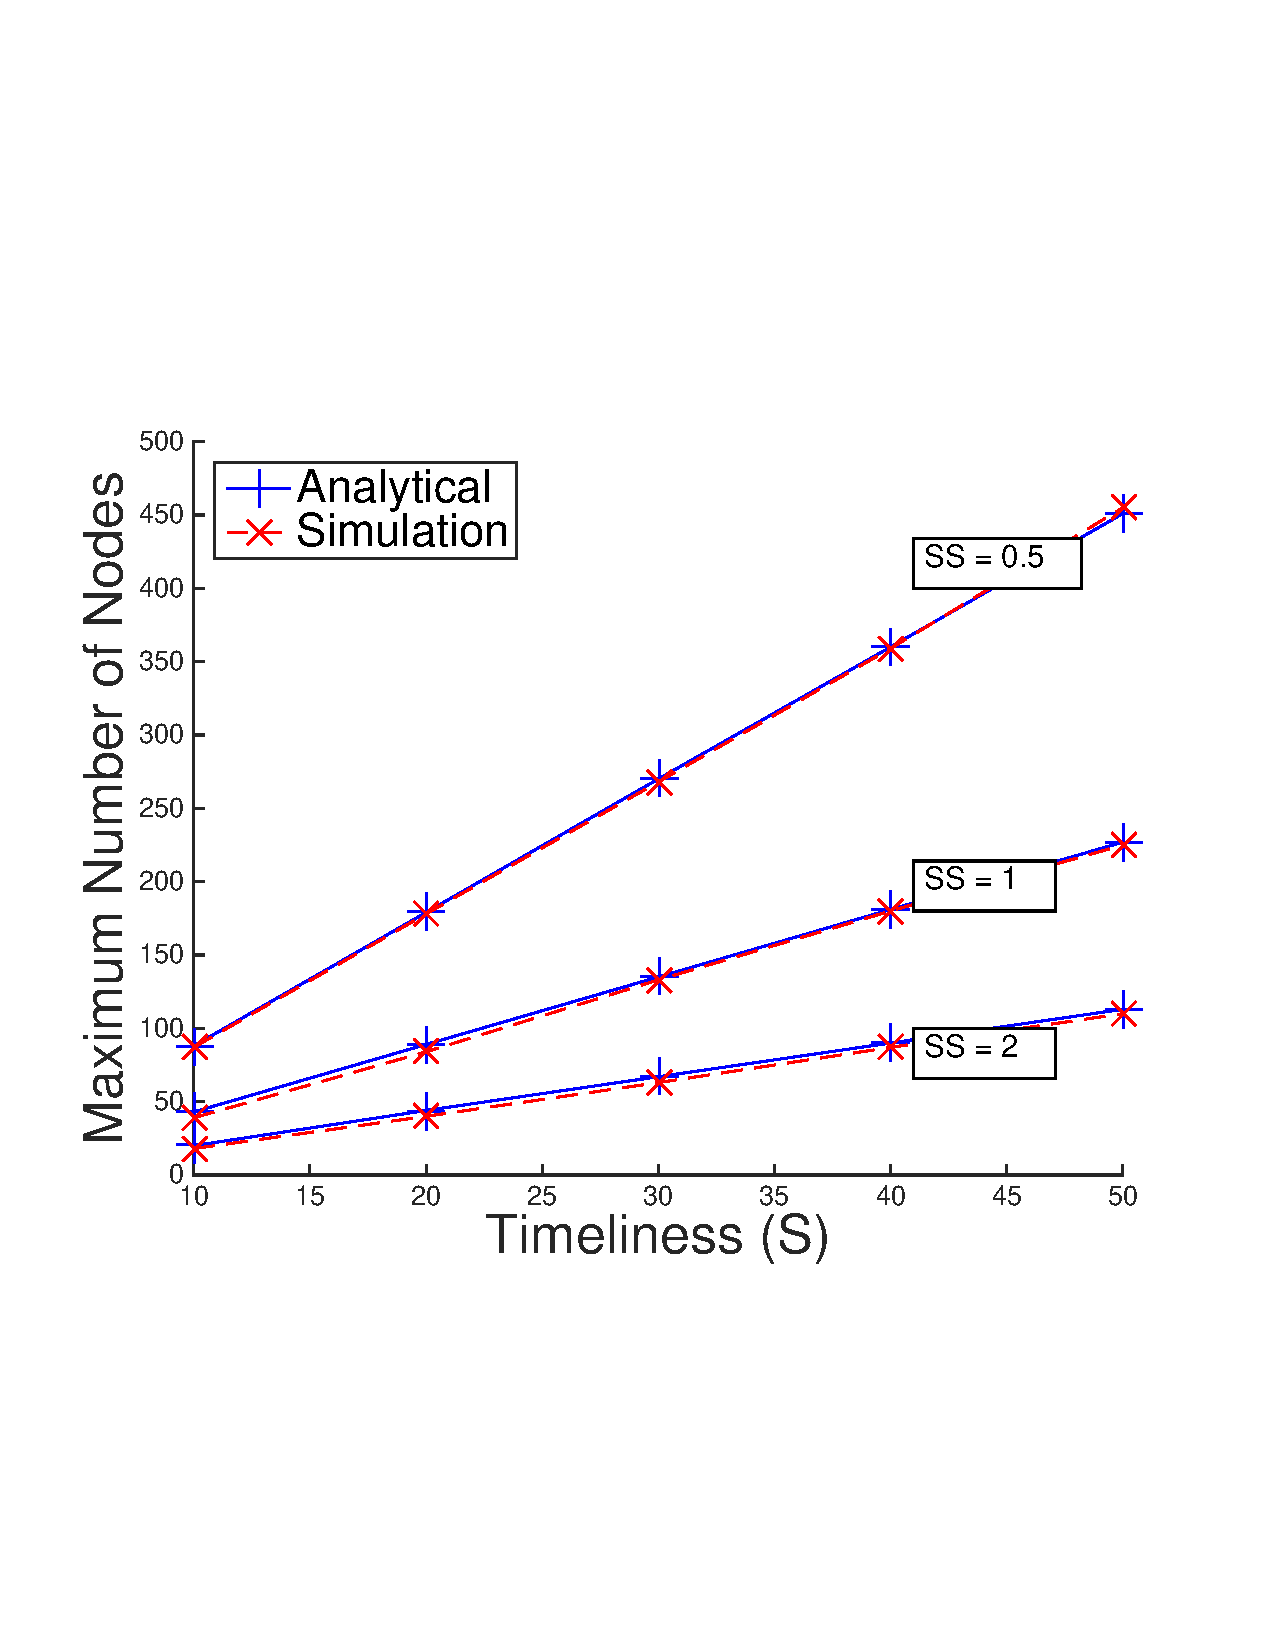
\includegraphics[scale=0.40, clip=true, trim=12mm 65mm 20mm 65mm]{figures/scal_sim_results/color_2d/line_uni_2d_qoi_vs_non_color_multiple.pdf}
        \label{fig:scal_vs_qoi_line}
        }
    \subfigure[Grid Network, $I_S = 48 KB$]{
%        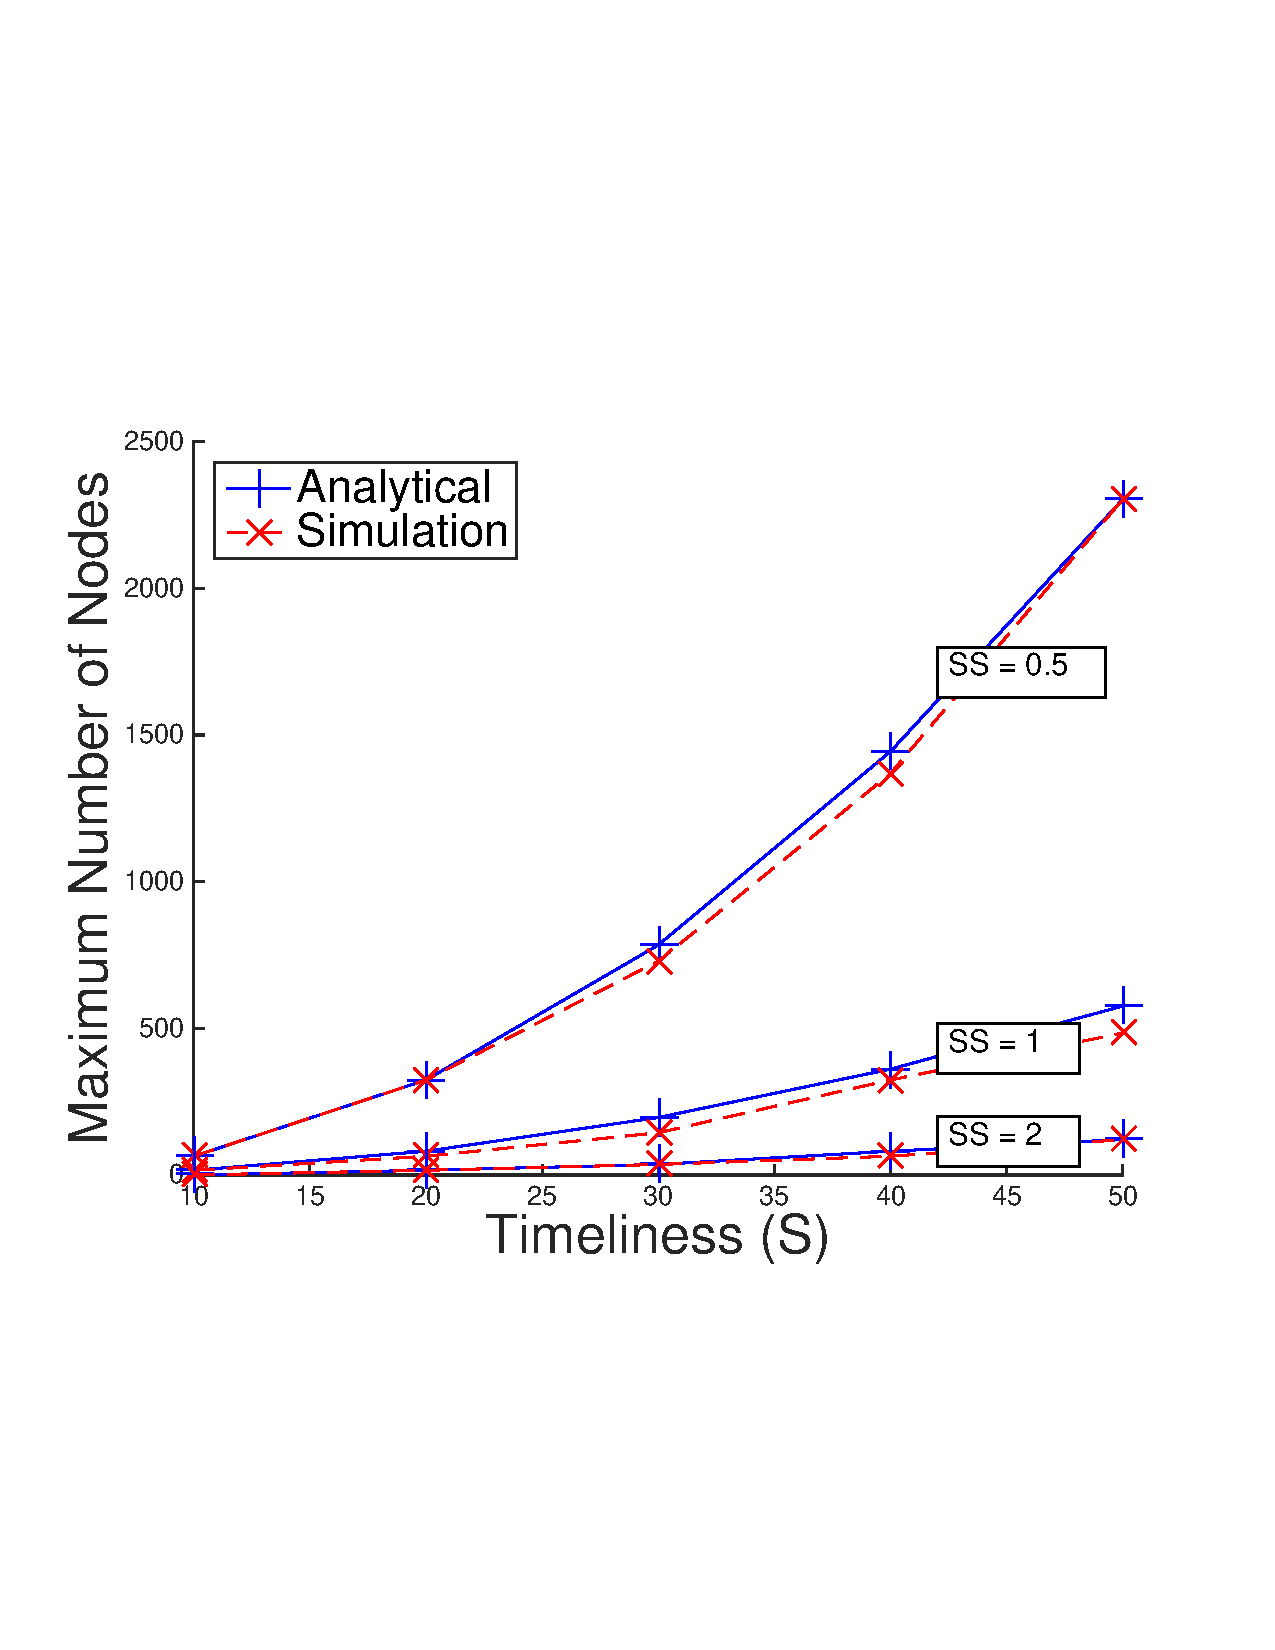
\includegraphics[scale=0.40, clip=true, trim=12mm 65mm 20mm 65mm]{figures/scal_sim_results/color_2d/grid_uni_2d_qoi_vs_non_color_multiple.pdf}        
        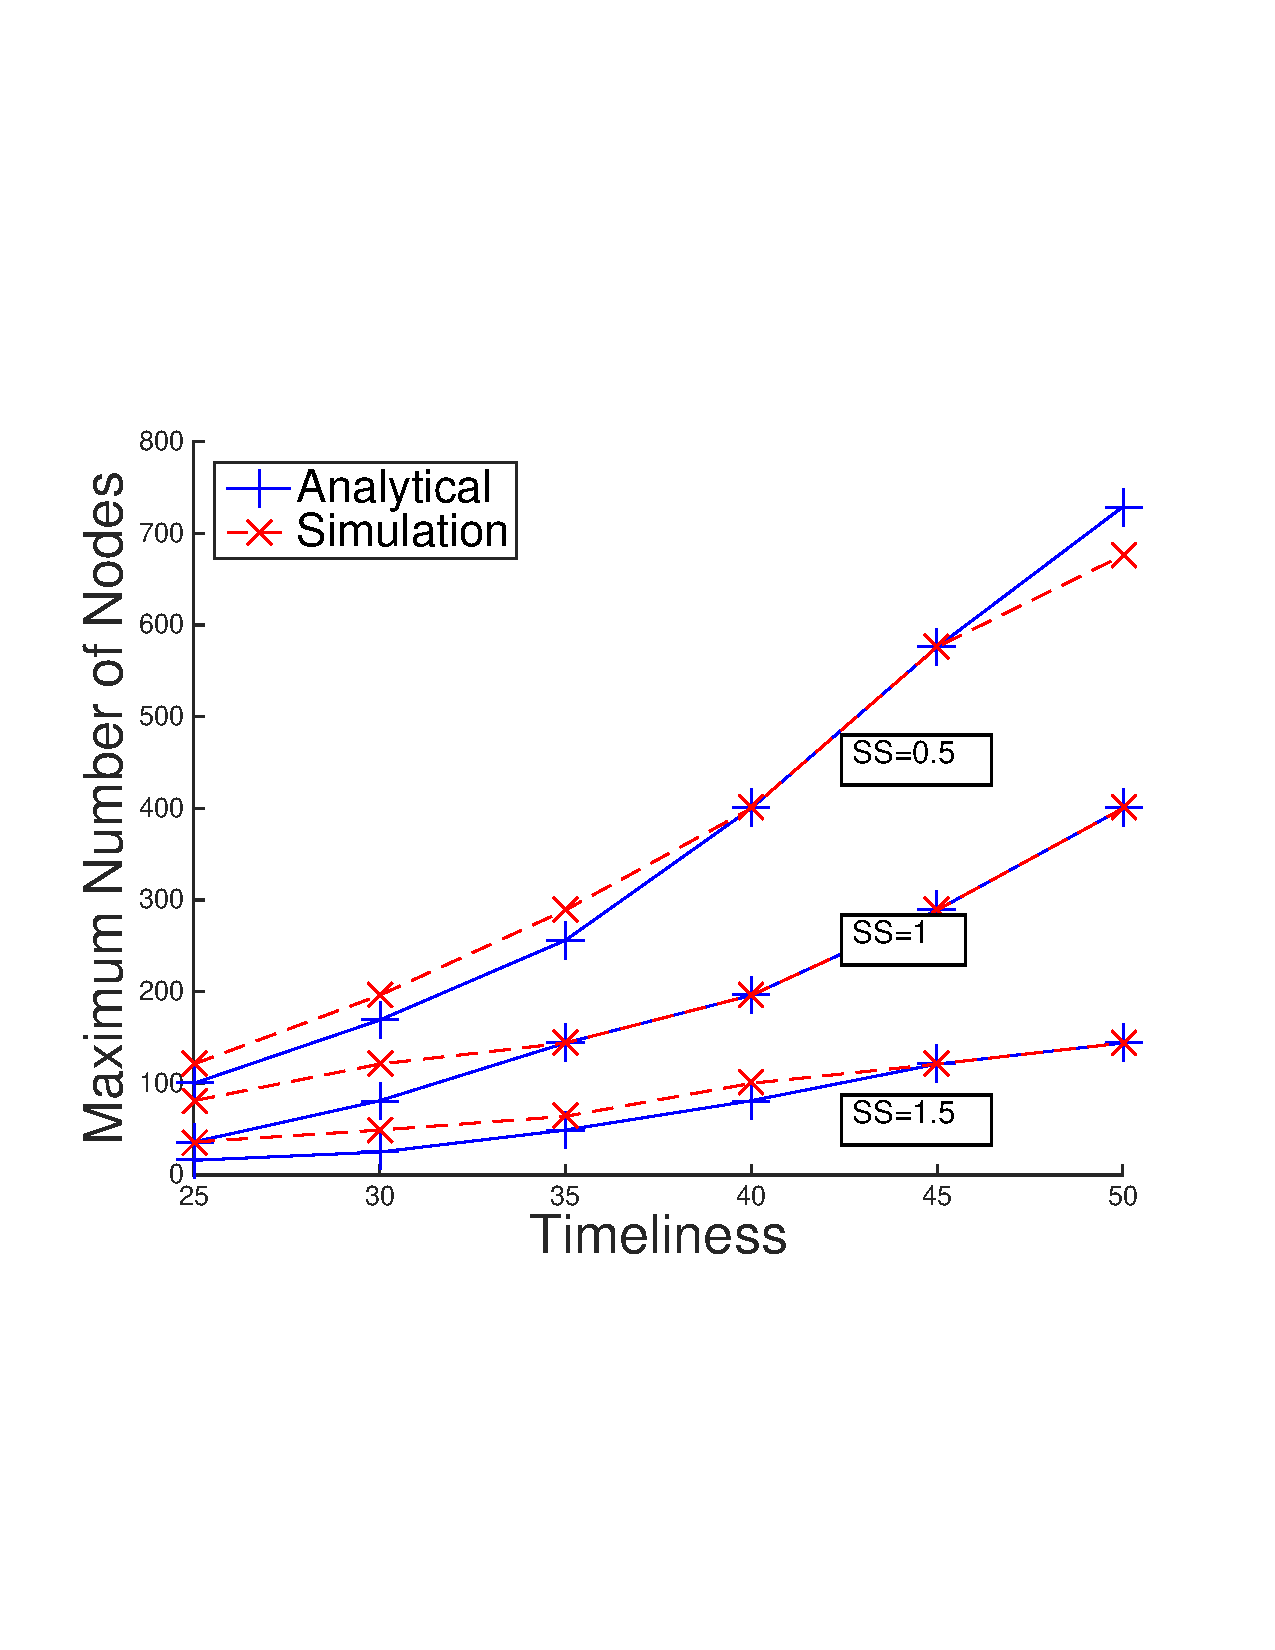
\includegraphics[scale=0.40, clip=true, trim=12mm 65mm 20mm 65mm]{figures/scal_sim_results/color_2d/grid_scal_chernoff.pdf}
        \label{fig:scal_vs_qoi_grid}
        }
   \caption{Empirical results match analytical results closely for all tests.}
   \label{fig:scal_vs_qoi}
\end{figure}

To show how effective estimates using this framework can be, we simulated the network topologies and traffic described above in Section \ref{sec:example_applications} in the ns3 network simulator, comparing empirical results to those generated analytically with this framework, labeled \emph{Analytical}.  The results of these simulations are shown in Figure \ref{fig:scal_vs_qoi}.
%Due to space concerns, we only show a subset of results in Figure \ref{fig:scal_vs_qoi} to provide evidence of the effectiveness of the methodology.  All results generated, however, exhibit very similar trends of proximity between empirical and the analytical values.
We use a channel rate of $W= 2 Mbps$, packet sizes of $P_s = 1500$ bytes, and image sizes of $18$ and $48$ Kbytes.  As above, the correlation between Sum Similarity and $k_{req}$ is taken from the actual observed relation in Figure \ref{fig:topkSumSim}.  All values of parameters ($SS$, $T$, $I_S$, etc.) were chosen to test a variety of network sizes and QoI requirements while remaining within realistic network sizes, both with respect to real-world deployments and simulations with feasible run-times.


